\chapter{Interface features:}
\section{First run}
The first time you launch \xlogo\ (or if you have deleted the file \texttt{.xlogo} - Read Section \ref{file_perso}), a dialog box will ask you for your language.
\begin{center}
 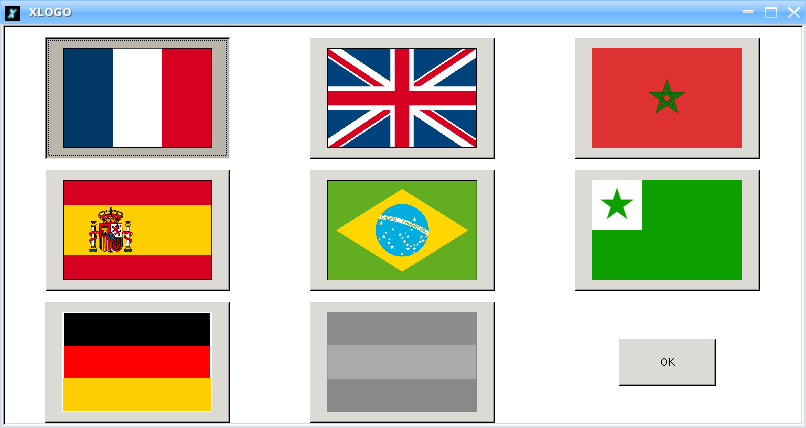
\includegraphics[scale=0.2]{pics/interface-CaptureLangue.png} 
\end{center}
Then, you could modify the language with the Preferences Dialog Box (Read Section \ref{general_tab}).
\section{The main window}
\begin{center}
 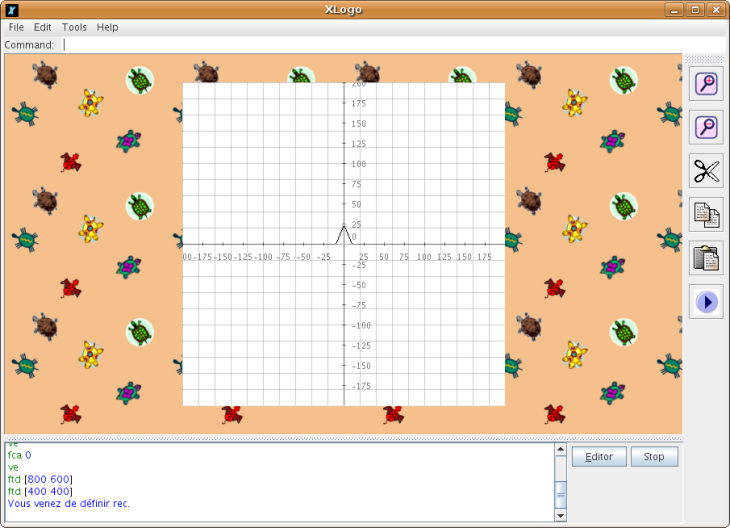
\includegraphics[  scale=0.4]{pics/interface-Capture.png} 
\end{center}

\begin{itemize}
\item Along the top, there are the usual menus \textbf{File Edit Options and Help}
\item Just below this is \textbf{the command line}, which allows the logo instructions
to be applied.
\item In the middle of the screen is \textbf{the drawing area}. 
\item On the right of the drawing area, a\textbf{ tool bar} allows the user to do several actions:
\begin{itemize}
\item Zoom in/out.
\item Edit (cut/copy/paste)
\item The ``play'' button launches the main command defined in the editor.
\end{itemize}
\item At the bottom is the \textbf{command history}, which shows every command entered, and the associated response. To quickly recall a command which has already been entered, there are two options: you can either click on the old command in the history, or you can click several times
on the upper scroll-arrow until the desired command appears. The upper and lower scroll-arrows in fact allow you to navigate through all
the commands that you have already entered (very practical). 
\item To the right of the history are two buttons: \textbf{STOP and EDITOR}. 
\begin{itemize}
 \item Button STOP interrupts the execution of the program.
\item Button EDITOR allows the procedure editor to be opened.\\ 
\end{itemize}
\end{itemize}
\section{The procedure editor}
\begin{center}
 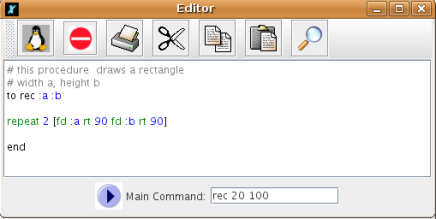
\includegraphics[scale=0.4]{pics/interface-CaptureEditor.png}
\end{center}
There are three ways to open the editor:\\
\begin{itemize}
\item Enter \texttt{ed} on the command line at the top of the screen. The
editor will then open to show all the procedures already defined.
If you only want to edit specific procedures, enter:\\
 \texttt{ed {[}procedure\_1 procedure\_2 $\ldots$]}
\item Press the Editor button on the main screen. 
\item Use the keyboard shortcut Alt+E. 
\end{itemize}
These are the different buttons that you will find in the editor:\\

\begin{longtable}{cm{12cm}}
 \includegraphics*[scale=1]{pics/interface-turtle.png} &
Save the changes made in the editor and then close it. It is this
button that you have to press each time you want to apply newly entered
operations. If you prefer, you can use the keyboard shortcut ALT+Q.\\
\includegraphics*[scale=1]{pics/interface-quit.png}&
Close the editor without saving any of the changes made there. You
can also use the shortcut ALT+C.\\
 \includegraphics*[scale=1]{pics/interface-fileprint.png}&
 Print the contents of the editor.\\
 \includegraphics*[scale=1]{pics/interface-editcopy.png}&
 Copy the selected text to the clipboard.\\
 \includegraphics*[scale=1]{pics/interface-editcut.png}&
 Cut the selected text to the clipboard.\\
 \includegraphics*[scale=1]{pics/interface-editpaste.png}&
 Paste the selected text from the clipboard.\\
 \includegraphics*[scale=1]{pics/interface-chercher.png}&
 Open a Replace/Find Dialog Box for the procedure Editor.\\
\end{longtable}
\begin{center}
 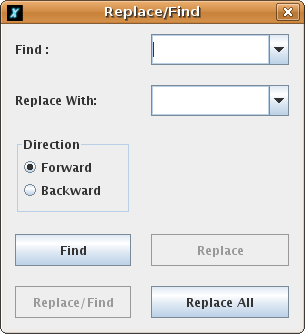
\includegraphics[scale=0.4]{pics/interface-CaptureFind.png}
\end{center}
\vspace{0.5cm}

\includegraphics{pics/interface-play.png}
At the bottom of the editor, a text field allows the user to define a main command. This command is the general instruction that launches the program. It can be accessed with the ``play'' button from the main window's tool bar. This command is saved and then restored when the editor and all its content are recorded in a Logo format file (\texttt{.lgo})\\ \\
\textbf{\begin{Large}IMPORTANT\end{Large}}: \\
\begin{itemize}
\item Note that clicking on the close button (x) in the window titlebar will have no effect! Only the two main buttons will allow you to quit
the editor. 
\item To delete one or more unwanted procedures, use the primitives \texttt{er} and \texttt{erall}, or use in the menu bar, Tools$\to$ Procedure Eraser.
\end{itemize}
\section{Quit \xlogo}
To quit \xlogo, you can choose in the menu bar, \textbf{File - Quit} or click on the close button in the window titlebar. A dialog box wil ask you if you really want to quit.
\begin{center}
 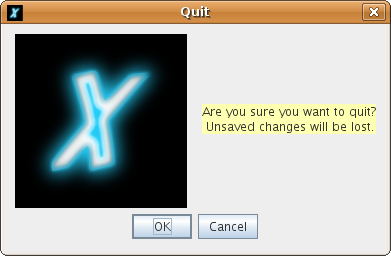
\includegraphics[scale=0.4]{pics/interface-CaptureQuit.png}
\end{center}
\chapter{Menu options:}
\section{``File'' Menu}
\begin{itemize}
\item \textbf{File$\to$New}: delete all procedures and variables. You create a new workspace.\\
\item \textbf{File$\to$Open}: open a previously saved logo file. 
\begin{center}
 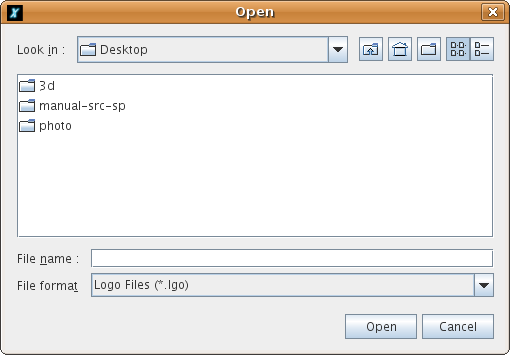
\includegraphics[scale=0.4]{pics/interface-CaptureOpen.png}
\end{center}
\vspace{0.25cm}
\item \textbf{File$\to$Save as...} save the current procedures under a different
name. 
\begin{center}
 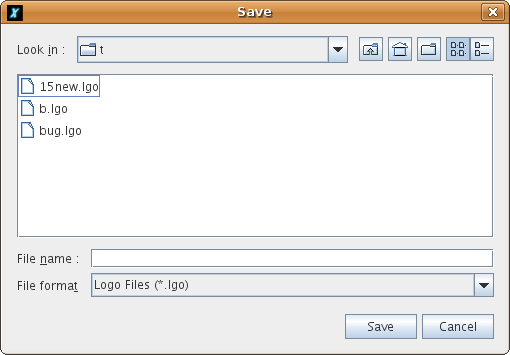
\includegraphics[scale=0.4]{pics/interface-CaptureSave.png}
\end{center}
\vspace{0.25cm}
\item \textbf{File$\to$Save}: save the procedures in the current file. \\
\item \textbf{File$\to$Capture image$\to$Save image as...} : allow the image to be
saved in jpg or png format. If you wish to select only a part
of the image, you can define a bounding box by dragging the mouse on the drawing area.
\vspace{0.25cm}
\item \textbf{File$\to$Capture image$\to$Print image}: allows the image to be printed.
In the same way as above, you can select an area to print. \\
\item \textbf{File$\to$Capture image$\to$Copy image into the clipboard}: put the image into the system clipboard. Just as for printing and recording, you can select an area of the image. This functionality works very well under the Windows environments. On the other hand, it does not work under Linux (the clipboard has a different behaviour).\\
\item \textbf{File$\to$Text$\to$Save As... (RTF) }: save the command history in RTF format (color and text format are preserved).\\
\item \textbf{File$\to$Quit}: quit the \xlogo\  application. 
\end{itemize}

\section{``Edit'' Menu}
\begin{itemize}
\item \textbf{Edit$\to$Copy}: copy the selected text to the clipboard. \\
\item \textbf{Edit$\to$Cut}: cut the selected text to the clipboard. \\
\item \textbf{Edit$\to$Paste}: paste the text contained in the clipboard into the command line.\\
\item \textbf{Edit$\to$Select All}: select all the text in the command line.
\end{itemize}

\section{``Tools'' Menu}
\begin{itemize}
 \item \textbf{Tools$\to$Pen Color}: allows the colour with which the turtle will draw to be chosen from a palette of colours. Also accessible
via the command \texttt{setpc}.
\begin{center}
 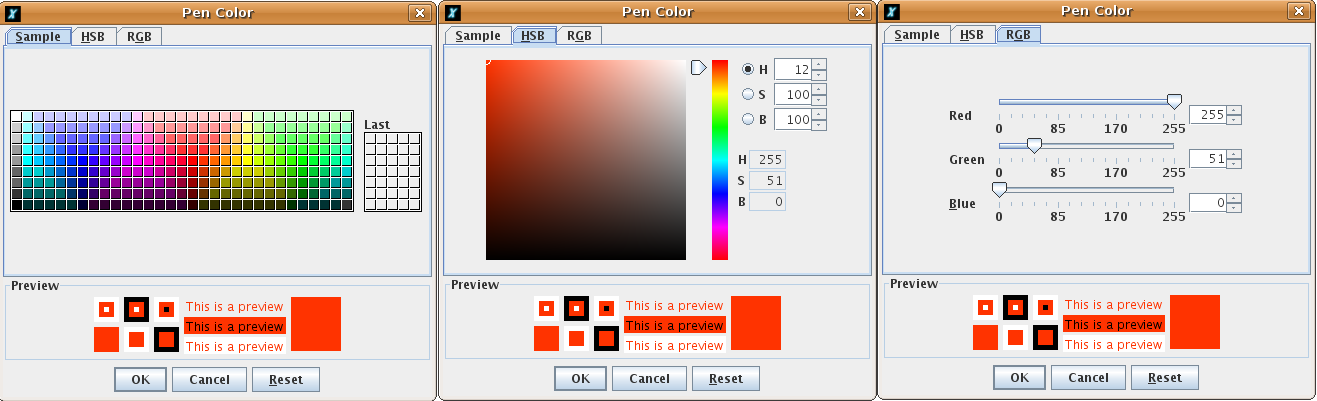
\includegraphics[scale=0.3]{pics/interface-CaptureColor.png}
\end{center}
\vspace{0.25cm}
\item \textbf{Tools$\to$Screen Color}: set the color of the screen background. Accessible via the primitive \texttt{setscreencolor}.\\
\item \textbf{Tools$\to$Start Up File}: allows the path to {}``start-up'' files to be defined. Any procedures contained in these {*}.lgo format
files will then become {}``pseudo-primitives'' in the \xlogo\ language. They cannot be edited or changed by the user. You can thus define
personalised primitives. 
\begin{center}
 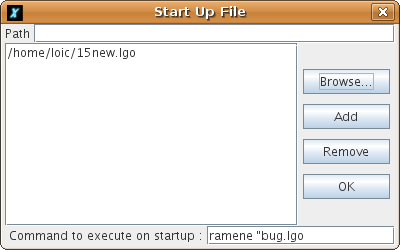
\includegraphics[scale=0.4]{pics/interface-CaptureStart.png}
\end{center}
\vspace{0.25cm}
\item \textbf{Tools$\to$Code Translator}: allows code translation from one language to another. In fact, very useful when you want to use an \xlogo\ example written in another language.
\begin{center}
 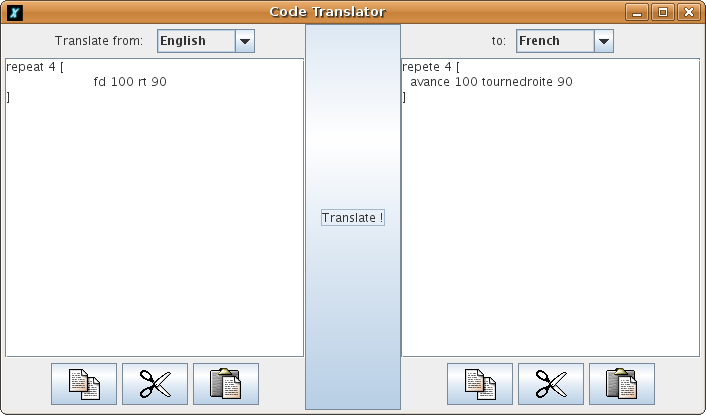
\includegraphics[scale=0.4]{pics/interface-CaptureTranslator.png}
\end{center}
\vspace{0.25cm}
\item \textbf{Tools$\to$Procedure Eraser}: with this dialog box, you can delete some procedures. You can also modify the order of appearance of the procedures in the editor.\\
\begin{center}
 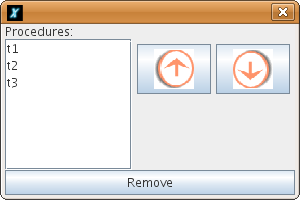
\includegraphics[scale=0.4]{pics/interface-CaptureProcedure.png}
\end{center}
\vspace{0.25cm}
\item \textbf{Tools$\to$Preferences}: opens a dialog box in which you can configure several things:
\begin{itemize}
\label{general_tab}
\item \textbf{General Tab:} 
	\begin{itemize}
	\item \textbf{Language} : allows language to be chosen. Note that the primitives differ in each language.
	\item \textbf{Look}: allows the {}``look'' or skin of \xlogo\ to be defined. Metal, Native Java and Motif styles are available.
	\item \textbf{Drawing speed}: if you prefer to see all the turtle's movements, you can slow it down by using the slider bar on the first tab.
	\end{itemize}. 
	\begin{center}
 		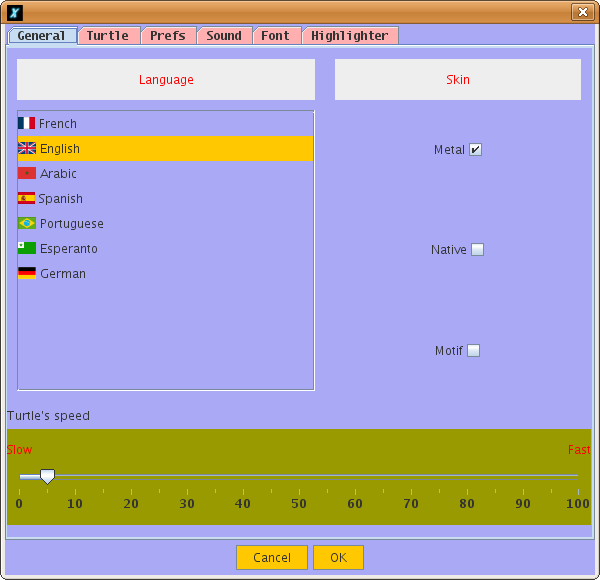
\includegraphics[scale=0.3]{pics/interface-CapturePref1.png}
 		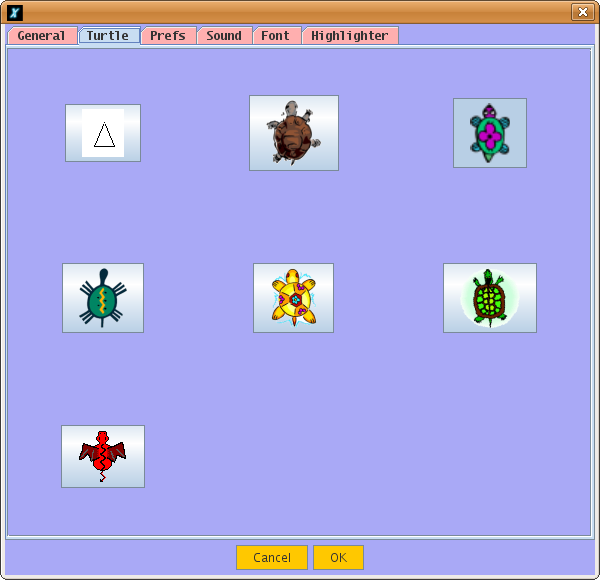
\includegraphics[scale=0.3]{pics/interface-CapturePref2.png}
	\end{center}
	\vspace{0.25cm}
\item \textbf{Turtle Tab}: On the second tab, you can choose your preferred turtle.
	\begin{center}
 		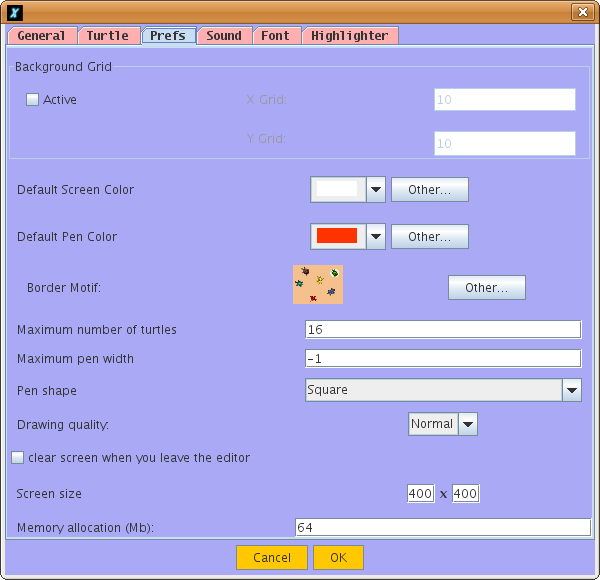
\includegraphics[scale=0.4]{pics/interface-CapturePref3.png}
	\end{center}
\item \textbf{Options Tab}: On the third tab, many options:\\
	\begin{itemize}
	\item \textbf{Background grid}: You can choose to draw a grid on the background drawing screen. You can define the width and the height of a square of the grid and the grid color.
	\item \textbf{Background axis}: You can choose to draw horizontal axis or vertical axis on the background drawing screen. You can define the distance between two divisions and the axis color.
	\item \textbf{Default screen color}: You can define a default screen color.
	\item \textbf{Default pen color}: You can define a default pen color.
	\item \textbf{Border motif}: You can choose your own motif for the drawing area's border (an image or a uniform color).
	\begin{center}
 		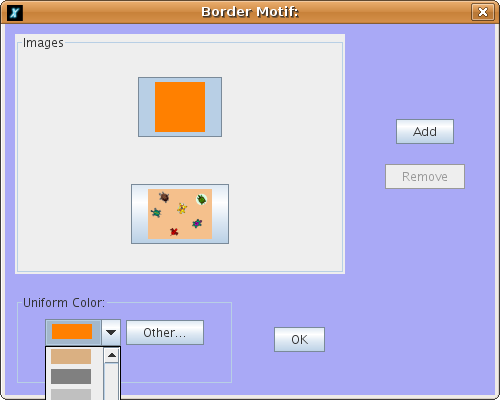
\includegraphics[scale=0.4]{pics/interface-CaptureBorder.png}
	\end{center}
	\item \textbf{Maximum pen width}: You can choose the maximum pen width allowed. If you don't want to use this option, put -1.\\
	\item \textbf{Pen shape}: You can choose the shape of the pen, round or square.\\
        \item \textbf{Drawing quality}: Finally, you can choose the accuracy of the drawing line. In high quality, pen edges will be smoothed. But remember that by increasing the quality you will lose some execution speed.
	\item \textbf{Maximum number of turtles}: You can choose the maximum number of turtles available in mode multiturtle.\\
	\item \textbf{Clear screen when closing the editor}: You can choose if you want to clear the screen when you leave the editor.
	\item \textbf{Clear variables when closing the editor}: You can choose if you want to clear all variables when you leave the editor. (And you restart working with a "clean" workspace)
	\item \textbf{Screen size}: You can choose a personal size for the drawing area. Default size is 1000 by 1000 pixels. Be careful, when you increase the size of the drawing area, you may need to increase the memory size of \xlogo, (an error message will pop up). 
        \item \textbf{Memory allocation:} You can change the memory space allocated to \xlogo. Default size is 64MB. You might have to increase this if you want to work on a bigger drawing area. If you modify this parameter, you must restart \xlogo\ so that the change takes place. \textcolor{red}{Be careful}, do not over increase this parameter since it could considerably slow your system down.
	\item \textbf{TCP port number}: You can modify the default TCP port used for networking. (See p.\pageref{network})
	\end{itemize}
	\begin{center}
 		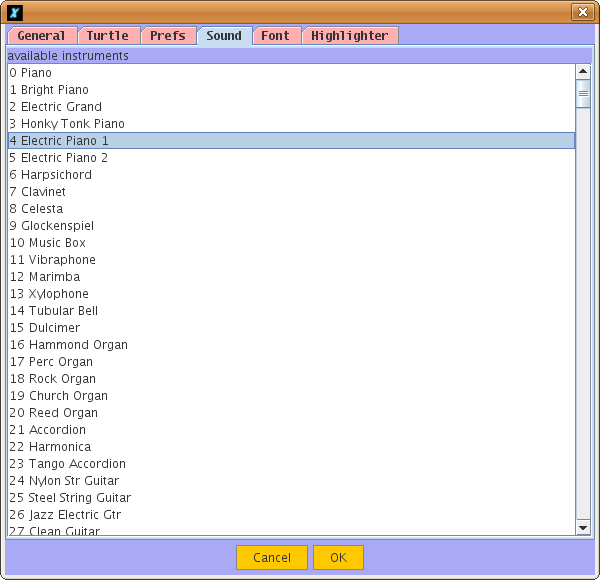
\includegraphics[scale=0.4]{pics/interface-CapturePref4.png}
	\end{center}
	\vspace{0.25cm}
\item \textbf{Sound Tab: }On the fourth tab, you can choose an instrument for your MIDI interface. If you experience some detection problems, and the list is empty, have a look at the FAQs at the end of the manual. This function can be accessed with the primitive \texttt{setinstrument}. 
	\begin{center}
 		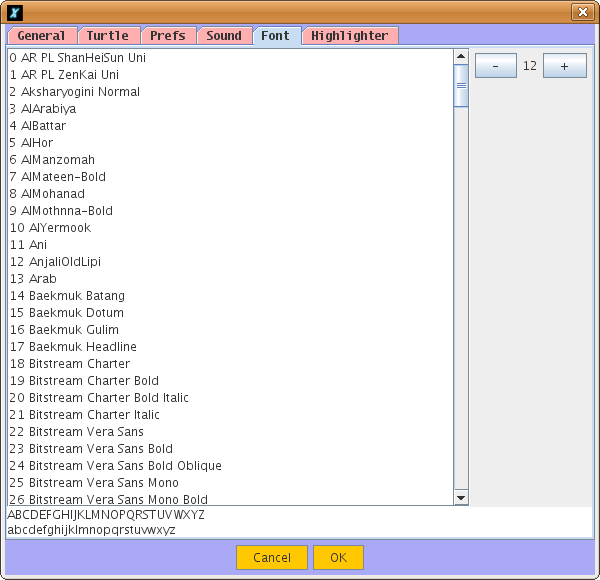
\includegraphics[scale=0.4]{pics/interface-CapturePref5.png}
	\end{center}
	\vspace{0.25cm}
\item \textbf{Font Tab}: On the fifth tab, you can choose the font for the interface.
	\begin{center}
 		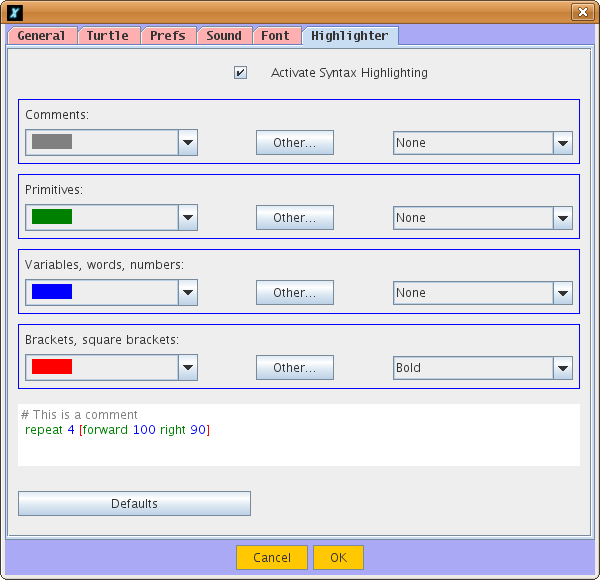
\includegraphics[scale=0.4]{pics/interface-CapturePref6.png}
	\end{center}
	\vspace{0.25cm}
	\item \textbf{Highlighter Tab}: You can choose active syntax highlighting and define your own highlight colors.
\end{itemize}
\end{itemize}
\section{``Help'' Menu}
\begin{itemize}
\item \textbf{Help$\to$Online Manual}: Displays the reference manual of \xlogo, accessible only by internet. 
	\vspace{0.25cm}
\item \textbf{Help$\to$Licence}: shows the GPL license under which this software is distributed.
	\begin{center}
 		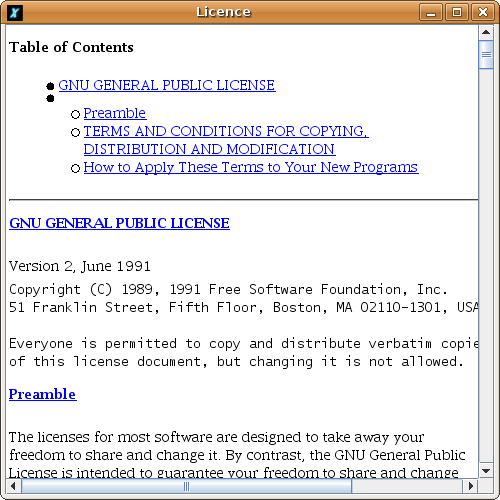
\includegraphics[scale=0.4]{pics/interface-CaptureLicence.png}
	\end{center}
	\vspace{0.25cm}
\item \textbf{Help$\to$Translation}: shows a translation of the above license. This translation has no official standing - this belongs only to the English version, and the translation is provided here only as an aid to understanding.

\item \textbf{Help$\to$Translate \xlogo}: this dialog box allows to consult/modify/complete \xlogo\ transaltions for any language (messages and primitives).\\
	\begin{center}
 		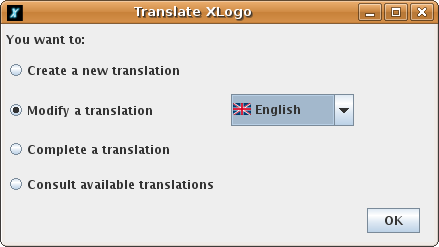
\includegraphics[scale=0.4]{pics/interface-CaptureXLogoTranslate1.png}
 		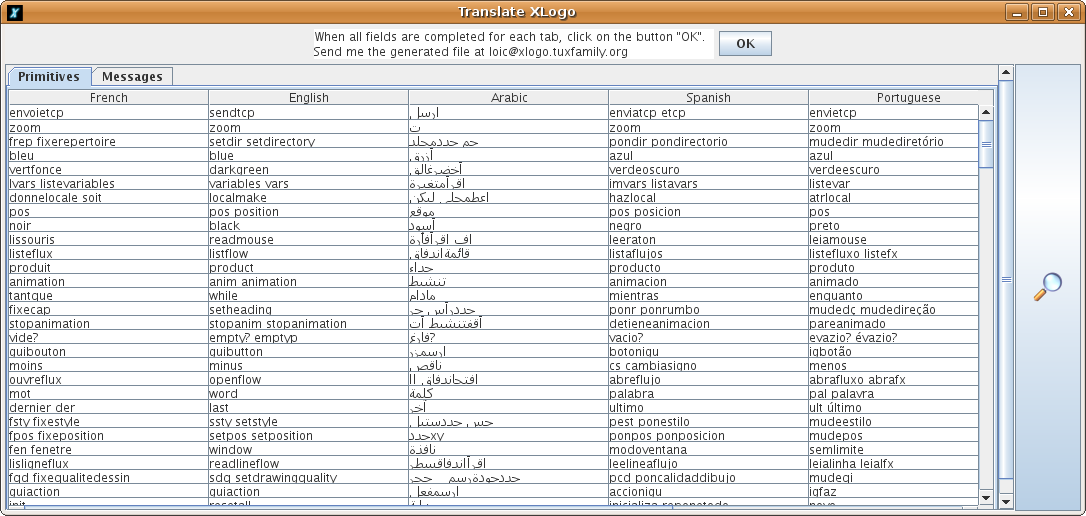
\includegraphics[scale=0.4]{pics/interface-CaptureXLogoTranslate2.png}
	\end{center}
	\vspace{0.25cm}
	Otherwise, You can create a new translation for a new language if you want to. In every case, send me the generated file at \texttt{loic@xlogo.tuxfamily.org}
\item \textbf{Menu -- > About}: The standard thing .... and xlogo.tuxfamily.org for your bookmarks !! o:) 
	\begin{center}
 		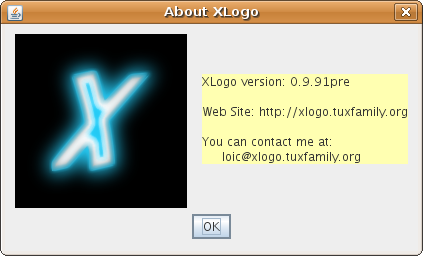
\includegraphics[scale=0.6]{pics/interface-CaptureAbout.png}
	\end{center}
	\vspace{0.25cm}
\end{itemize}
